\documentclass[letterpaper, 11pt]{article}
\usepackage{latexsym}
\usepackage{amssymb}
\usepackage{times}
%\usepackage[in]{fullpage}
\usepackage{amsmath,amsfonts,amsthm}
\usepackage{graphicx}

%\documentclass[11pt]{article}
%\pagestyle{myheadings}
%\usepackage[ruled,nothing]{algorithm}
%\usepackage{algorithmic}
%\usepackage[dvips]{epsfig,graphicx}
%\numberwithin{equation}{section}

\bibliographystyle{plain}

\newenvironment{newalgo}[2]{\begin{algorithm}

\caption{\textsc{#1}}\label{#2}

\begin{algorithmic}[1]}{\end{algorithmic}\end{algorithm}}



\newcommand{\gm}{\gamma}
\newcommand{\wh}{\widehat}
\newcommand{\rep}{representation}
\newcommand{\rv}{random variable}
\newcommand{\la}{\lambda}
\newcommand{\wt}{\widetilde}
\newcommand{\st}{such that}
\newcommand{\slvary}{slowly varying}
\newcommand{\ma}{moving average}
\newcommand{\regvary}{regularly varying}
\newcommand{\asy}{asymptotic}
\newcommand{\ts}{time series}
\newcommand{\id}{infinitely divisible}
\newcommand{\seq}{sequence}
\newcommand{\fidi}{finite dimensional \ds}

\newcommand{\ble}{\begin{lemma}}
\newcommand{\ele}{\end{lemma}}
\newcommand{\bfX}{{\bf X}}
\newcommand{\pro}{probabilit}
\newcommand{\BX}{{\bf X}}
\newcommand{\BY}{{\bf Y}}
\newcommand{\BZ}{{\bf Z}}
\newcommand{\BV}{{\bf V}}
\newcommand{\BW}{{\bf W}}
\newcommand{\reals}{{\mathbb R}}
\newcommand{\bbr}{\reals}

\newcommand{\balpha}{\mbox{\boldmath$\alpha$}}
\newcommand{\bbeta}{\mbox{\boldmath$\beta$}}
\newcommand{\bmu}{\mbox{\boldmath$\mu$}}
\newcommand{\tbmu}{\mbox{\boldmath${\tilde \mu}$}}
\newcommand{\bEta}{\mbox{\boldmath$\eta$}}


\def \br#1{\left \{#1 \right \}}
\def \pr#1{\left (#1 \right)}

\newcommand{\Gm}{\Gamma}
\newcommand{\ep}{\epsilon}


\newtheorem{lemma}{Lemma}[section]
\newtheorem{figur}[lemma]{Figure}
\newtheorem{theorem}[lemma]{Theorem}
\newtheorem{proposition}[lemma]{Proposition}
\newtheorem{definition}[lemma]{Definition}
\newtheorem{corollary}[lemma]{Corollary}
\newtheorem{example}[lemma]{Example}
\newtheorem{exercise}[lemma]{Exercise}
\newtheorem{remark}[lemma]{Remark}
\newtheorem{fig}[lemma]{Figure}
\newtheorem{tab}[lemma]{Table}
\newtheorem{fact}[lemma]{Fact}
\newtheorem{test}{Lemma}
\newtheorem{algorithm}[lemma]{Algorithm}

\newcommand{\play}{\displaystyle}

\newcommand{\ms}{measure}
\newcommand{\beao}{\begin{eqnarray*}}
\newcommand{\eeao}{\end{eqnarray*}\noindent}
\newcommand{\beam}{\begin{eqnarray}}
\newcommand{\eeam}{\end{eqnarray}\noindent}
\usepackage{hyperref}

\newcommand{\halmos}{\hfill\mbox{\qed}\\}
\newcommand{\fct}{function}
\newcommand{\ins}{insurance}
\newcommand{\ds}{distribution}

\newcommand{\one}{{\bf 1}}
\newcommand{\eid}{\buildrel{\rm d}\over {=}}
\newcommand {\Or}{\rm ORDER}
\newcommand {\In}{\rm INTER}

\newcommand{\bbd}{{\mathbb D}}
\newcommand{\vi}{$V_{ij}$ }
\newcommand{\rr}{R^{\prime\prime}}
%\newcommand{\R}{R^\prime}
\newcommand{\ci}{\frac{1}{c}}
\newcommand{\Vi}{V(n)}
\newcommand{\dR}{\mathcal R}
\newcommand{\md}[1]{\left(\ \rm{mod}\ \it{#1}\right)}
\newcommand{\So}{s}
%\begin{document}
%\def\DoubleSpace{\baselineskip=24pt}
%\DoubleSpace \sloppy

\begin{document}



\title{Modulo7 - A Semantic and Technical Analysis of Music and Lyrics
\\} 
\author{\textbf{Arunav Sanyal, Aakash Bhambhani}}
\maketitle

%%%%%%%%%%%%%%%%%%%
\section*{Abstract}
The web contains a vast pleathora of music translated into text format. Musical repositories include lyrics, chord charts, note sequences, sheet music etc. Moreover there are many software available on the web to convert songs into frequency distributions, from which we can obtain information on the sound engineering aspects of songs.\\\\
While individual software exists which addresses some of these issues, there is no holistic framework in existence which addresses all of these concerns to present a comprehensive analysis of music. We present an implementation "Modulo7" which attempts to address some of these issues. You can find the source code of Modulo7 here \href{https://github.com/Khalian/Modulo7}{\textbf{MODULO 7 SOURCE CODE}}
 \\\\
Modulo7 has multiple features. 
\begin{enumerate}
\item A \textbf{web crawler} which obtains lyrics and note contains by parsing lyrics sites.
\item A \textbf{lyrics analyzer} which takes input from user a few sentences and returns a recommendation or a rank ordering of the songs similarity parsed in step one of the songs and the user input sentences.
\item A \textbf{note analyzer} which analyses mood and tonal content of the song and perform song recommendation based on music theory concepts.
\item A \textbf{frequency analyzer} that takes a file with actual frequencies and converts them into evenly spaced musical notes in ad standard scale and standard key.
\end{enumerate} 

\section*{Music Theory Concepts}
Western music is represented by 7 basic notes A B C D E F G and 5 accidentals(notes in between basic notes) A\#, C\#, D\#, F\#, G\#. (No notes in between B,C and E, F) These 12 notes taken together can express almost every piece of western music (we don't consider the exceptions in Modulo7). The following are some terminologies in music theory:
\begin{enumerate}
\item The leap/spacing between any two consecutive notes is called a \textbf{semitone}. For example a leap from A to A\# or from B to C is moving one semitone up. 
\item A note one semitone below a basic note is called a \textbf{flat} denoted by symbol b following the note. This is another kind of accidental .For instance Ab, Db etc. Its important to note that certain notes are "equivalent". For instance G\# is exactly the same as Ab in which pitch it expresses. This is called \textbf{harmonic equivalence}. For the purpose of our analysis we standardized all accidentals to sharps. 
\item The number of semitones that separate any two arbitrary notes is called the \textbf{interval} between these notes. For example there are two semitones in between A and B so the interval is 2. Similarly there are 3 semitones in between A and C so the interval is 3. In theory these intervals have fancy names(with particular meaning and affect to listener) which we will elaborate of the note analysis section.
\item The \textbf{Key} of a song refers to the base note on which a song is played and only has subjective meaning. Transposing a song to a different key means moving every note of the song across a fixed interval.
\item The \textbf{Scale} of a song refers a set of sequences (interval distances) between the key and other notes of a song. There are many scales each with its distinctive "emotional" expression.
\end{enumerate} 

We have made the following assumptions for the purpose of our analysis.
\begin{enumerate}
\item We consider simple monotonic melody lines (one note followed by another). Concepts like harmony (notes stacked on each other/ multiple notes played at one) are not taken into account.
\item We have ignored existence of quarter notes (pitches in between any two notes) to keep analysis of intervals simple.
\item We use both scale information and interval counts (explained in note analyzer part) to judge mood content of a song.
\item We dont consider phrasing aspects (time difference between successive notes) or rhythm aspects of a song.
\end{enumerate}

\section*{Crawler}
Our crawler code fetches links to various lyrics/note pages and then iteratively crawls through each song page to create a notestream file and a lyrics file respectively. Due to the non standardized nature of lyrics sites we have chosen http://keylessonline.com/ for testing. The site provides note and lyrics information in a single page per song, making the job of parsing easier. \\\\
The Crawler works as follows:-
\begin{enumerate}
\item User calls build\_song\_sources\_crawler.pm. This will crawl to the root page of the lyrics site and fetch all links. It only keeps the links which point to western music representations of the song. This list is stored in a file called song\_sources.txt
\item User then calls music\_source\_crawler.pm. This will read song\_sources.txt and retrieve the pages of the songs. It then extracts the notes and lyrics contents of the file. For each song it generates two files - the notestream file (.nsf) and lyrics file (.lyrics). The note stream file contains the key and the scale of the song followed by the series on notes that the song plays in sequence. The lyrics file contains text only pertaining to the lyrics of the song. These files are further used by the note analyzer and lyrics analyzer respectively. 
\end{enumerate}

\section*{Note Analyzer}
The note analyzer is called via note\_analyzer.pm. It reads the notestream files created by buildSongSources.pm and then generates interval frequency vectors. The description of these vectors are given in the interval analysis subsection.
\subsection*{Interval Analysis}
Each interval between two notes gives a distinct tone to the song. For instance an interval = 1  is called "minor second" which gives a tense sadness to the tone. Similarly interval = 7 is called a "perfect fifth" which gives a sense of power to the tone. Similarly different intervals express different moods. \\\\
Our interval analysis part leverages the relative frequencies of the intervals in the song. Given a note stream, we can calculate the intervals between every two successive notes. We then count the frequency of each interval and store it into a interval frequency vector. This creates a basic vector space of songs. 
\subsection*{Mood Analysis}
Now after the interval interval frequency vector space is generated, we can perform various analysis on top of it. For instance we can codify hand crafted rules to ascertain the genre of the song. For instance a prevalance of perfect fifths is a strong indication of the song being a rock song. Similarly a predominance of minor intervals (minor thirds, minor seconds etc) can classify the song as being sad. \\\\
In order to quantify these analyses we define three objective measures:-
\begin{enumerate}
\item Happiness index : The fraction of major intervals in the song. The more major intervals there are (2, 4, 6), the more happier the song sounds. 
\item Sadness index : The fraction of minor intervals in the song. The more minor intervals there are (1, 3, 5), the more sadder the song sounds. 
\item Power index : The fraction of perfect intervals in the song. The more perfect intervals there are (7, 8), the more neutral/power the tone projects. For example rock songs have a disproportionately higher number of perfect fifths (interval = 7) in them.
\item Tension index : The fraction of interval = 6 in songs. This leads to an unresolved, tense tone in the song. This interval is very rarely seen in songs.
\end{enumerate}
We also take into account the scale of the song. The scale is directly acquired by the crawler while parsing the lyrics site. However if the scale is not listed, we assume its a minor scale since it is the most commonly occurring scale in music. (the method required to estimate the key of a song from its note requires advanced concepts of music theory which is out of scope of this project). We add a small weight to the index depending on the scale (for major scale add weight to happiness index and similarly for minor scale add weight to sadness index). \\\\
We present this analysis to the user. Qualitatively user can compare the four indices to judge what mood the song presents. Note this does not take into account which parts of the song express what mood, its a rather coarse analysis.

\subsection*{Song recommendation}
Based on the interval frequencies we can perform song recommendation. The recommendation follows two steps
\begin{enumerate}
\item All songs are standardized to a single key('a') by a process of key transposition. Moreover each note stream is converted to note frequency vectors, forming a vector space model. 
\item A song is picked by the user. The recommender then computes the cosine similarities of user picked song with all songs are presents a ranked order of songs. Based on number of relevant songs desired by the user a list(recommendation) is presented.
\end{enumerate}

\section*{Lyrics Analyzer}
We have created a lyrics analyzer(lyrics\_analyzer.pm) that acts as a ranking engine/recommender system based on user input. From the output of the ".lyrics" file from the crawler, the note analyzer reads files and constructs the lyrics frequency vectors of the songs. The lyrics frequency vector omits various stop words, which are ad hoc coded by the authors. \\\\
These frequency vectors form a vector space and are analogues to the doc vectors present from homework 2. Now the program asks from user some input text. These can be lines from a song the user likes or some words that the user prefers to be present in the song(effectively an intent of the user of what he/she wishes to view in the songs recommended by the recommender). The user also presents the number of relevant songs he/she wishes to see. \\\\
The lyrics analyzer then computes cosine similarity of all the songs lyrics frequency vectors with the query and then presents the user specified number of relevant songs to the user. 

\section*{Frequency Analyzer}
We have taken a set of 50 songs in the form of .mp3 files for this part of the project. We use a program called "Sonic Visualiser" with an added plugin called "Melodia" to extract the high frequency vocal content from the song. \\\\ This plugin traverses the entire audio data and evaluates raw frequency values over very small intervals, which are in the order of 3 milliseconds (thus we have one frequency value for evry 3 milliseconds). This can be saved to a simple plain text file. We have written a perl program to aggregate the frequencies to a larger interval of 0.25 seconds (else we will have files spanning 80,000 entries including noise and outliers) and convert the aggregated frequency into musical notes considering standard tuning.\\\\We know that the lyrics will be followed only by the vocals in the song and the lyrics themselves are not directly related to any other parameter of the song. This is the reason we wish to analyze the vocals because not only are the vocals directly following the lyrics, but they are directly influenced by other aspects of the song such as the chords, key notes, major/minor scale, etc. Also from our study of basic signal processing we know that the vocals will be a part of the high frequency portion of songs and performing simple Fourier transformations over small batches of the high frequency components of the song will give us a discrete frequency which will in essence represent the vocals. Now the perl program will convert these frequencies into evenly spaced notes.\\\\The musical system on a standard tuning of 440 Hz starts with the C note which has a frequency of 16.35 Hz. The next note is the C\# (C-sharp) note which has a frequency of 17.32 Hz, and so on D - 18.35, D\# - 19.45, E - 20.60, F - 21.83, F\# - 23.12, G - 24.50, G\# - 25.96, A - 27.50, A\# - 29.14 and B - 38.87. This is the first octave starting at C$_0$ and ending at B$_0$. In the second octave, all the frequencies will be doubled ie. C$_1$ will be equivalent to C$_0$ * 2. In the third octave all frequency values will be double the corresponding frequency values in the second octave and so on. Thus we try to find the closest possible match to the aggregated frequency and replace it with its corresponding note. This result is then provided to the notes analyzer to evaluate power index and other such metrics for each song.

\section*{Experimental Evaluation and Results}
We have performed the following experiments on the different components of Modulo7.
\begin{enumerate}
\item For the crawler we crawled the list on http://keylessonline.com/list/hindi which presents 86 different links to parse. Our crawler then parsed all these into separate notestream and lyrics files. The note stream files are perfectly generated, but the lyrics stream files contains the occasional non lyrics words. This happens as the html page does not distinguish between lyrics and non lyrics words, hence the parser relies on omitting words like "album" and "copyright" (an analogous to a stopword list for lyrics). The crawler both sets of files in .nsf and .lyrics files.
\item For the lyrics analyzer, we parsed the set of songs from the .lyrics file and then we provide an interactive querying system. The user can judge subjectively whether the returned results are relevant or not. 
\item For the notes analyzer, we parsed the set of songs from the .nsf files and then performed mood analysis on it. All 86 songs are bollywood songs (and none of them are rock songs so we dont expect high power indices). \\\\
We present the \textbf{average mood indices} for both the output of frequency\_analyzer and the web crawler:-
\begin{center}
\textbf{FOR BOLLYWOOD SONG SET : OUTPUT OF CRAWLER}
\begin{tabular}{ |c|c| } 
 \hline
 Happiness Index & 0.159 \\ 
 Sadness Index & 0.21 \\ 
 Power Index & 0.105 \\ 
 Tension Index & 0.0082\\ 
 \hline
\end{tabular}
\end{center}
\begin{center}
\textbf{FOR ECLECTIC SONG SET : OUTPUT OF FREQ ANALYZER}
\begin{tabular}{ |c|c| } 
 \hline
 Happiness Index & 0.168 \\ 
 Sadness Index & 0.19 \\ 
 Power Index & 0.14 \\ 
 Tension Index & 0.007\\ 
 \hline
\end{tabular}
\end{center}
From our experiments we are able to ascertain that the power index is low (on average 0.1) for the bollywood songs which is correct since they are not rock songs. But its higher since the eclectic song set cuts accross genres. This evaluation can be done best by running the interactive menu of notes\_analyzer.pm.
\item For frequency analysis, we have taken 50 different songs from eclectic sources. All the songs are in the form of .mp3 files (downloaded via iTunes). These songs are analyzed by the plugin to produce a set of 50 .txt files which represent the raw frequency samples. This is used as the input for the perl code which aggregates and converts the raw frequencies into a stream of notes thus generating a set of 50 .nsf files which can then be passed to the notes analyzer. For e.g. taking a song Skyfall sung by Adele we perform frequency analysis. We have the following graph before the frequency analysis:\\\\
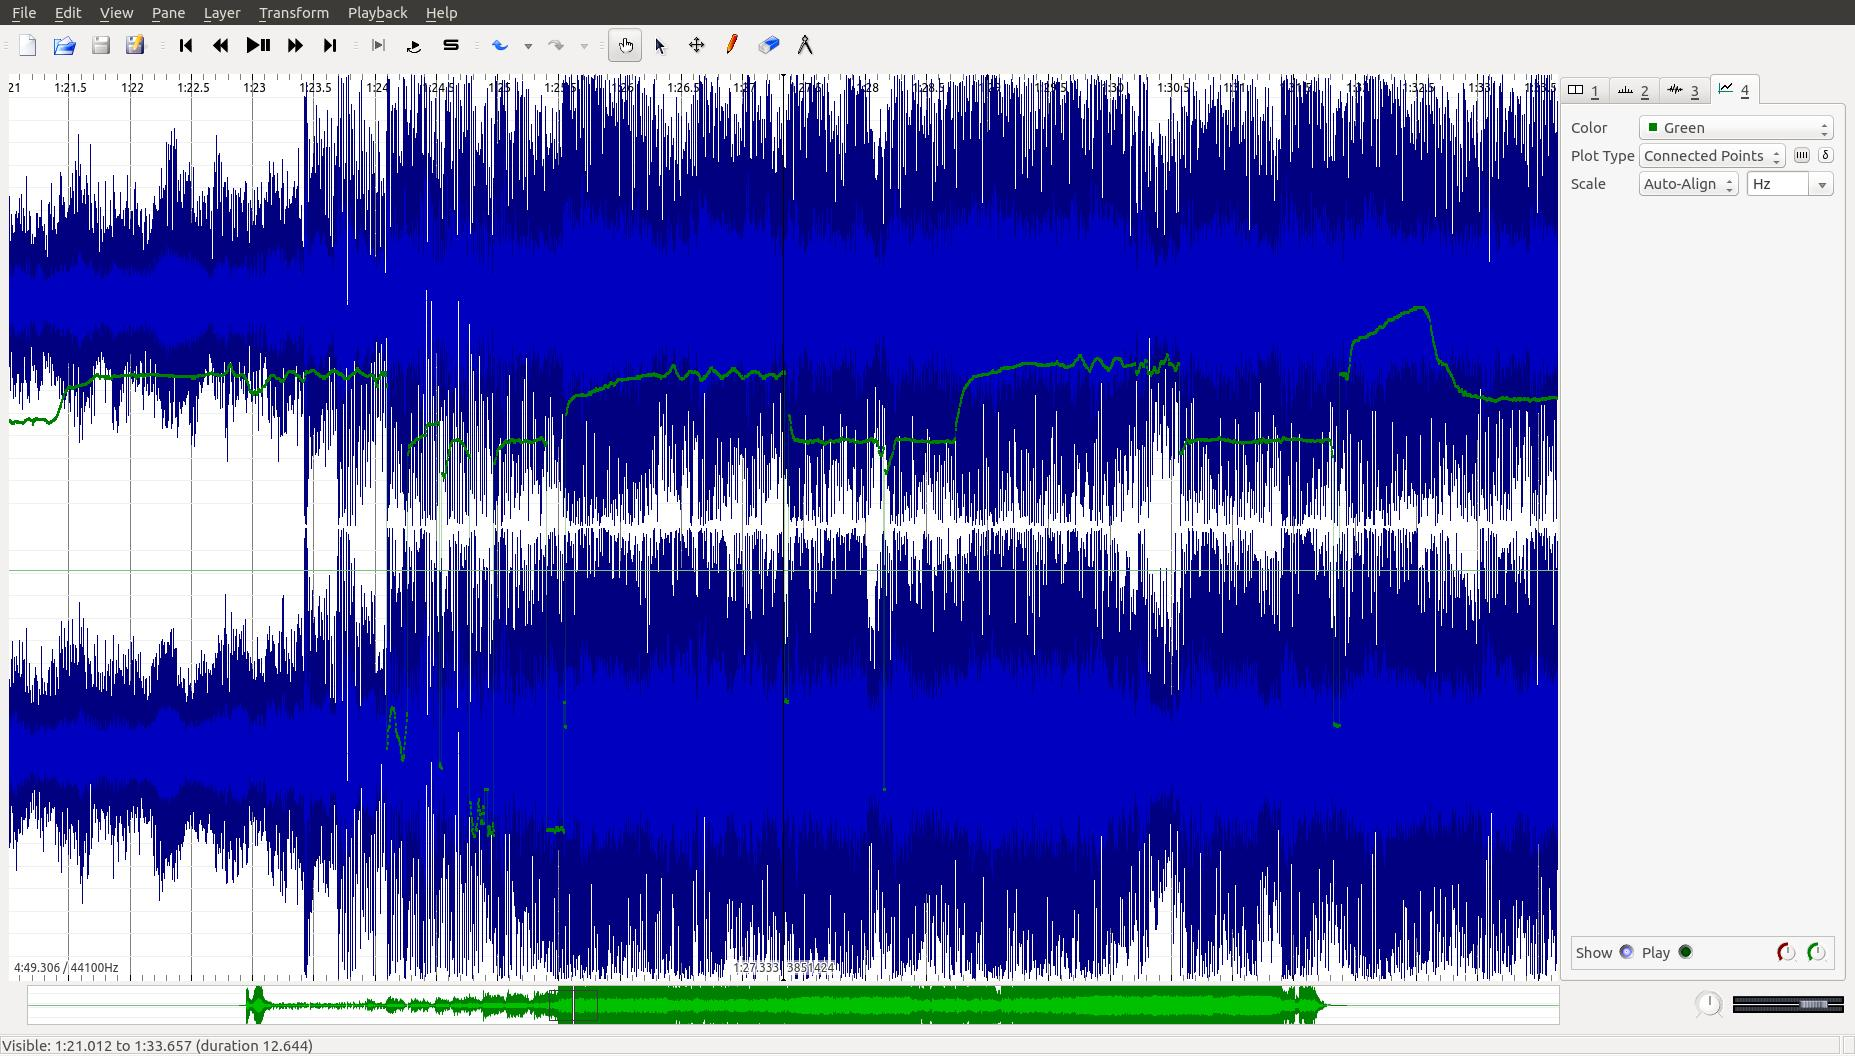
\includegraphics[width=\textwidth]{after.jpg}\\\\
The blue area represents the cumulative of all audio content, the upper data being the left channel and lower data being the right channel. The green line in the middle of the upper data represents the vocal frequency that has been extracted from the song (upper because the vocals seem to be present in the left channel in this case). Playing just the raw frequency extracted gives a crude but very accurate tone of the vocals.
\end{enumerate}

\section*{Contributions by individual members on the project}
\begin{enumerate}
\item \textbf{Arunav Sanyal} Created the crawler, lyrics analyzer and frequency analyzer components.
\item \textbf{Aakash Bhambhani} Created the frequency analyzer component and its integration with the frequency analyzer.  
\end{enumerate}
\end{document}

%%%%%%%%%%%%%%%%%%%%%%%%%%%%%